\documentclass[handout]{beamer}

\usetheme[progressbar=frametitle]{metropolis}
\metroset{block=fill}

\subtitle{NTIN071 Automata and Grammars}
\author{Jakub Bulín (KTIML MFF UK)}

\date{Spring 2025\\ 
    \vspace{1in} 
    \begin{flushleft}
        \it \footnotesize * Adapted from the Czech-lecture slides by Marta Vomlelová with gratitude. The translation, some modifications, and all errors are mine.
    \end{flushleft}
}

%% packages

\usepackage{amsmath}
\usepackage{amssymb}
\usepackage{amsthm}
\usepackage{cancel}
\usepackage{color}
\usepackage{colortbl}
\usepackage{forest}
\usepackage[utf8x]{inputenc}
\usepackage{multicol}
\usepackage{multirow}

%% colors
\definecolor{Gray}{gray}{0.9}

%% TikZ
\usepackage{tikz}
    \usetikzlibrary{
        automata,
        arrows,
        backgrounds,
        decorations.pathmorphing,
        fit,
        positioning,
        shapes,
        shapes.geometric,
        tikzmark
    } 
    \tikzset{>=stealth',shorten >=1pt,auto,node distance=2cm}
    \tikzset{initial text={}}
    \tikzset{elliptic state/.style={draw,ellipse}}

%% amsthm
\theoremstyle{plain}
    \newtheorem*{algorithm}{Algorithm}    
    \newtheorem*{observation}{Observation}
    \newtheorem*{proposition}{Proposition}

\theoremstyle{remark}
    \newtheorem*{exercise}{Exercise}
    \newtheorem*{remark}{Remark}

%% macros
\DeclareMathOperator{\RegE}{RegE}
\DeclareMathOperator{\RL}{RL}

% Just for Lecture 2
\newcommand{\x}{$\times$}
\newcommand{\nx}{\ }



\title{Lecture 9 -- Closure properties of context-free languages, Dyck languages}


\begin{document}


\frame{\titlepage}


\begin{frame}{Recap of Lecture 8}
	
    \begin{itemize}
        \item Pushdown automata accept exactly context-free languages (constructions: CFG to PDA and PDA to CFG)
        \item A deterministic pushdown automaton (DPDA)
        \item DPDA recognize a proper subclass of context-free languages,\\ accepts by empty stack iff prefix-free and accepts by final state\\
        (Deterministic PDA + acceptance by empty stack does not even cover regular languages!)
        \item Deterministic PDA have unambiguous grammars
        \item The landscape of languages
        \item Converting between representations of context-free languages
        \item Undecidable problems about context-free languages (preview)
	\end{itemize}

\end{frame}


\section*{2.12 Closure properties of context-free languages}


\begin{frame}{Closed under union, concatenation, iteration, reverse}

    \begin{theorem}
        If $L,L'\subseteq\Sigma^*$ are context-free, then so are $L\cup L'$, $L.L'$, $L^*$, $L^+$, $L^R$.
    \end{theorem}
    \textbf{Proof:} Let $G,G'$ be CFG generating $L,L'$ such that $V\cap V'=\emptyset$. Take a new start symbol $S_{new}\notin V\cup V'$.
        
    \begin{itemize}
        \item \alert{union} $L\cup L'$: add the rule $S_{new}\rightarrow S_1\mid S_2$
        \item \alert{concatenation} $L.L'$: add $S_{new}\rightarrow S_1S_2$
        \item \alert{iteration} $L^*$: add $S_{new}\rightarrow SS_{new}\mid\epsilon$
        \item \alert{positive iteration} $L^+$: add $S_{new}\rightarrow SS_{new}\mid S$           
        \item \alert{reverse} $L^R$: reverse the bodies of all production rules \\(i.e., $A\to\beta$ becomes $A\to\beta^R$)\hfill\qedsymbol
    \end{itemize}

\end{frame}


\section*{Substitution and homomorphism}


\begin{frame}{Recall the definitions}
   
    A (string) \alert{substitution} is a mapping $\sigma\colon \Sigma^*\rightarrow \mathcal P(Y^*)$ where
    \begin{itemize}
        \item $\Sigma$ and $Y$ are finite alphabets, $Y=\bigcup_{x\in \Sigma}Y_x$
        \item for each $x\in \Sigma$, $\sigma(x)$ is a language over $Y_x$
        \item $\sigma(\epsilon)=\{\epsilon\}$ and $\sigma(u.v)=\sigma(u).\sigma(v)$
    \end{itemize}
    For a language $L\subseteq \Sigma^*$, $\alert{\sigma(L)}=\bigcup_{w\in L}\sigma(w)\subseteq Y^*$. %A substitution is \alert{$\epsilon$-free} if no $\sigma(x)$ contains $\epsilon$.

    A (string) \alert{homomorphism} is defined similarly but each letter is mapped to a single word, $h\colon\Sigma^*\rightarrow Y^*$ where $h(x)\in Y_x^*$ for $x\in\Sigma$, $h(\epsilon)=\epsilon$ and $h(u.v)=h(u).h(v)$. Then \alert{$h(L)=\{h(w)\mid w\in L\}$}. %It is \alert{$\epsilon$-free} if $h(x)\neq\epsilon$ for all $x\in\Sigma$.

    The \alert{inverse homomorphism} applied to a language $L'\subseteq Y^*$: 
    $$
    h^{-1}(L')=\{w\in\Sigma^*\mid h(w)\in L'\}
    $$

\end{frame}


\begin{frame}{Example: substitution}
    
    \begin{example}
    Consider $G=(\{E\},\{a,+,(,)\},\{E\rightarrow E+E\mid (E)\mid a\},E)$. Let us have the following substitution:
    \begin{itemize}
        \item $\sigma(a)=L(G_a)$, where 
        \vspace{-3pt}
        $$
        G_a=(\{I\},\{a,b,0,1\},\{I\rightarrow I0\mid I1\mid Ia\mid Ib\mid a\mid b\},I)
        $$
        \vspace{-18pt}
        \item $\sigma(+)=\{-,*,:, \div, \mod\}$
        \item $\sigma(()=\{(\}$
        \item $\sigma())=\{)\}$
    \end{itemize}
    \end{example}
    Take $(a+a)+a\in L(G)$. Note that $(a+a)+a \notin \sigma(L(G))$, because $+\notin\sigma(+)$. But e.g. $(a001-bba)*b1 \in \sigma((a+a)+a)\subseteq\sigma(L(G))$

    \smallskip

    What if we modify the definition: $\sigma(\alert{(})=\{\alert{(},\alert{[}\}$, $\sigma(\alert{)})=\{\alert{)},\alert{]}\}$?

\end{frame}

  
\begin{frame}{Example: homomorphism}
        
    \begin{columns}

        \column{0.5\textwidth}
    
        \begin{example}
            $G=(\{E\},\{a,+,(,)\},$ $\{E\rightarrow E+E\mid (E)\mid a\},E)$        
            \begin{itemize}            
                \item $h(a)=\epsilon$
                \item $h(+)=\epsilon$
                \item $h(()=left$
                \item $h())=right$               
            \end{itemize}
        \end{example}
        \begin{itemize}
            \item $h((a+a)+a)=leftright $,
            \item $h^{-1}(leftright)\ni (a++)a$.
        \end{itemize}

        \vspace{1.75cm}
    
        \column{0.5\textwidth}

        \begin{example}
            $G=(\{E\},\{a,+,(,)\},$ $\{E\rightarrow a+E\mid (E)\mid a\},E)$
            \begin{itemize}
                \item $h_2(a)=a$
                \item $h_2(+)=+$
                \item $h(()=\epsilon$
                \item $h())=\epsilon$
            \end{itemize}
        \end{example}
        Are the following regular?
        \begin{itemize}
            \item $L(G)$
            \item $h(L(G))$
            \item $h^{-1}(h(L(G)))$
        \end{itemize}
        Is $h^{-1}(h(L(G)))=L(G)$?       
        
    \end{columns}
            
\end{frame}


\begin{frame}{Closure under substitution and homomorphism}
   
    \begin{theorem}
        Let $L\subseteq\Sigma^*$ be a context-free language.
        \begin{enumerate}[(i)]
            \item If $\sigma$ is a substitution on $\Sigma$ such that $\sigma(a)$ is context-free for all $a\in \Sigma$, then $\sigma(L)$ is context-free.
            \item If $h$ is a homomorphism on $\Sigma$, then $h(L)$ is context-free.
        \end{enumerate}   
    \end{theorem}

    \textbf{Idea:} replace terminals $a\in T$ in a parse tree with corresponding  parse trees for $\sigma(a)$ or $h(a)$, respectively

    \vspace{-12pt}
    \begin{multicols}{2}

        \phantom{.}

        \textbf{Proof:} \alert{(ii)} follows immediately from (i), define $\sigma(a)=\{h(a)\}$

        \alert{(i)} construct a context-free grammar for $\sigma(L)$ [next slide]

        
        \begin{center}
            \scalebox{1}{
                \input{files/subst.pdf_t}        
            }
        \end{center}

    \end{multicols}
    
\end{frame}


\begin{frame}{Proof: construct the grammar for $\sigma(L)$}

    Let us have the following context-free grammars, assume all their variable sets are disjoint:
    \begin{itemize}
        \item $G=(V,T,\mathcal P,S)$ generating $L$
        \item $G_a=(V_a,T_a,\mathcal P_a,S_a)$ generating $\sigma(a)$, for $a\in T$
    \end{itemize} 

    Construct a grammar $G'=(V',T',\mathcal P',S')$ where
    \begin{itemize}
        \item $V'=V\cup (\bigcup_{a\in T} V_a)$
	    \item $T'=\bigcup_{a\in \Sigma} T_a$
	    \item $\mathcal P'=(\bigcup_{a\in \Sigma} P_a) \cup \mathcal P''$ where $\mathcal P''$ is obtained from $\mathcal P$ by replacing every terminal $a$ by the variable $S_a$
	    \item $S'=S$
    \end{itemize}
    Clearly, $G'$ generates the language $\sigma(L)$.
    \hfill\qedsymbol

\end{frame}


\begin{frame}{Example}

    Consider the language
    $$
    L=\{a^ib^j\mid 0\leq i\leq j\}
    $$
    and the following substitution:
    \begin{itemize}
        \item $\sigma(a)=L_a=\{c^id^i\mid i\geq 0\}$
        \item $\sigma(b)=L_b=\{c^i\mid i\geq 0\}$
    \end{itemize}

    The grammars $G$, $G_a$, and $G_b$:
    \begin{itemize}
        \item $S\rightarrow aSb\mid Sb\mid\epsilon$\\
        \item $S_a\rightarrow c S_a d\mid\epsilon$
        \item $S_b\rightarrow c S_b\mid\epsilon$
    \end{itemize}
   
    Then the grammar $G'$ for $\sigma(L)$ consists of the following rules:
    $$
    S\rightarrow S_aSS_b\mid SS_b\mid\epsilon,\qquad S_a\rightarrow cS_ad\mid\epsilon,\qquad S_b\rightarrow cS_b\mid\epsilon
    $$

\end{frame}


\begin{frame}{Closure under inverse homomorphism}
    
    \begin{theorem}
        Let $L\subseteq Y^*$ be a context-free language and $h\colon\Sigma^*\to Y^*$ a homomorphism. Then $h^{-1}(L)$ is also context-free. Moreover, if $L$ is deterministic, then so is $h^{-1}(L)$.
    \end{theorem}

    \begin{columns}

        \column{0.5\textwidth}

        \textbf{Idea:} simulate a PDA $M$ for $L$

        \begin{itemize}
            \item read a letter $a$ $\Rightarrow$ place  $h(a)$ into an inner buffer
            \item simulate $M$, but with input taken from the buffer
            \item if buffer empties, read the next letter from real input
            \item accept iff empty buffer and $M$ is in accepting state
        \end{itemize}

        \column{0.5\textwidth}

        \vspace{-10pt}

        \begin{center}
            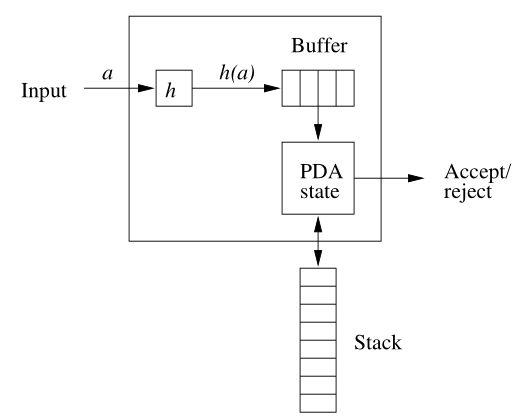
\includegraphics[width=\textwidth]{files/invHomoCFL.PNG}
        \end{center}

        \vspace{-15pt}

        \textbf{NB:} buffer is \alert{finite} $\Rightarrow$ can be encoded in the states:\\
        \alert{state} = (state, buffer contents)
        
    \end{columns}

\end{frame}


\begin{frame}{Proof: the construction}    
    
    Let $M=(Q,Y,\Gamma, \delta, q_0,Z_0,F)$ (by final state).
    We define a PDA  
    $$M'=(Q',\Sigma,\Gamma,\delta',\left[q_0,\epsilon\right], Z_0,F\times\{\epsilon\})$$ 
    where the set of states is the following ($u$ is the buffer)
    $$
    Q'=\{\left[q,u\right]\mid q\in Q, u\in Y^*, (\exists a\in \Sigma) (\exists v\in Y^*)\ h(a)=vu\}
    $$
    and the transition function is defined as follows:
    \begin{itemize}
        \item \alert{{[re]}fill buffer:} 
        \vspace{-6pt}
        $$
        \delta'(\left[q,\epsilon\right],a,Z)=\{(\left[q,h(a)\right],Z)\}
        $$
        \item \alert{read from buffer:}
        \begin{align*}
            \delta'(\left[q,u\right],\epsilon,Z)=&\{(\left[p,u\right],\gamma)\mid (p,\gamma)\in \delta(q,\epsilon,Z)\}\\
            \mathbin{\cup}&\{(\left[p,v\right],\gamma)\mid (p,\gamma)\in \delta(q,b,Z), u=bv\}
        \end{align*}
    \end{itemize}
 
    
    \medskip
    
    For a DPDA $M$, the resulting $M'$ is also deterministic.
    \hfill\qedsymbol

\end{frame}


\section*{Closure properties: it's complicated}


\begin{frame}{CFLs not closed under intersection}

    \begin{example}
        $L=\{0^n1^n2^n \mid n\geq 1\}=\{0^n1^n2^i \mid n,i\geq 1\}\cap \{0^i1^n2^n \mid n,i\geq 1\}$
    \end{example}

    $L$ is not context-free, even though both operands of the intersection are context-free:
 
    $L_1=\{0^n1^n2^i\mid n,i\geq 1\}$ generated by $G=(\{S,A,B\},\{0,1\},\mathcal P,S)$ with production rules 
    $$
    \mathcal P=\{S\rightarrow AB, A\rightarrow 0A1\mid\epsilon, B\rightarrow 2B\mid\epsilon \}
    $$
        
    $L_2=\{0^n1^n2^i \mid n,i\geq 1\}$ generated similarly using production rules 
    $$
    \mathcal P=\{S\rightarrow AB, A\rightarrow 0A\mid\epsilon, B\rightarrow 1B2\mid\epsilon \}
    $$

\end{frame}


\begin{frame}{Simulating two PDAs in parallel}

    Regular languages are closed under intersection, because we can simulate two DFAs in parallel. Why not PDAs?

    \begin{itemize}
        \item the FA units can be merged (same as for DFAs)
        \item reading input can be merged (one automaton can wait)
        \item but two stacks cannot be simulated on one stack!
    \end{itemize}
        
    In fact, `PDAs with two stacks' are equivalent to \alert{Turing machines}, can recognize any \alert{recursively enumerable} language $L\in{\mathcal L}_0$.

    \medskip
    \vdots
    \medskip

    But what if one of the PDAs does not really use its stack?

\end{frame}


\begin{frame}{Intersection of a context-free and a regular language}

    \begin{theorem}
        Let $L$ be a context-free language and $R$ a regular language. Then $L\cap R$ is context free. Moreover, if $L$ is deterministic, so is $L\cap R$.
    \end{theorem}

    \textbf{Proof:} Let $L=L(P)$ for a PDA $P=(Q_1,\Sigma,\Gamma,\delta_1,q_1,Z_0,F_1)$ and $R=L(A)$ for a DFA $A=(Q_2,\Sigma,\delta_2,q_2,F_2)$. Construct a PDA 
    $$
    M=(Q_1\times Q_2,\Sigma,\Gamma,\delta, (q_1,q_2),Z_0,F_1\times F_2)
    $$ 
    where we have a transition $\delta((q_1,q_2),a,X)\ni((r_1,r_2),\gamma)$ iff either
    \begin{enumerate}[(i)]
        \item $a\neq\epsilon$ and $(r_1,\gamma)\in \delta_1(q_1,a,X)$ and $r_2=\delta_2(q_2,a)$, or
        \item $a=\epsilon$ and $(r_1,\gamma)\in \delta_1(q_1,\epsilon,X)$ and $r_2=q_2$
    \end{enumerate}
    In (i) both automata read input, in (ii) $P$ works on its stack while $A$ waits. Clearly, $L(M)=L(P)\cap L(A)$ ($P$ and $R$ run in parallel).\hfill\qedsymbol       

\end{frame}


\begin{frame}{An application: proving non-context-freeness}

    \begin{example}
        $L=\{0^i1^j2^k3^\ell\mid i=0 \text{ or }j=k=\ell\}$ is not context-free.
    \end{example}
    
    \vspace{-6pt}
    By contradiction, assume $L$ is context-free.

    \smallskip
    The language $L_1=\{01^j2^k3^\ell \mid i,j,k\geq 0\}$ is regular (e.g. a regular grammar $\{S\rightarrow 0B, B\rightarrow 1B\mid C, C\rightarrow 2C\mid D, D\rightarrow 3D\mid\epsilon\}$.

    \smallskip
    But $L\cap L_1=\{01^i2^i3^i\mid i\geq 0\}$ is not context-free, a contradiction with the previous theorem.
    \hfill\qedsymbol

    \vspace{3pt}
    In fact, $L$ is a \alert{context-sensitive} language:    
    
    {\small
    \begin{columns}

        \column{0.48\linewidth}

        $S\rightarrow \epsilon\mid 0\mid 0A\mid B_1\mid C_1\mid D_1$\\
        $A\rightarrow 0\mid 0A\mid P$, $P\rightarrow 1PCD \mid  1CD$\\
        $B_1\rightarrow 1\mid 1B_1\mid C_1$\\
        $C_1\rightarrow 2\mid 2C_1\mid D_1$\\
        $D_1\rightarrow 3\mid 3D_1$
        
        \column{0.32\linewidth}

        \alert{$DC\rightarrow CD$} rewrite
        as\\ 
        context-sensitive rules\\
         $DC\rightarrow XC$, $XC\rightarrow XY$,\\ 
         $XY\rightarrow CY$, $CY\rightarrow CD$\\
        \phantom{.}
        
        \column{0.13\linewidth}

        $1C\rightarrow 12$\\
        $2C\rightarrow 22$\\
        $2D\rightarrow 23$\\
        $3D\rightarrow 33$\\
        \phantom{.}        
        
    \end{columns}
    }

\end{frame}


\begin{frame}{CFLs are not closed under difference nor complement}

    \begin{theorem}
        The class of the context-free languages is not closed under difference, nor complement.
    \end{theorem}

    \textbf{Proof:} $L_1\cap L_2=\overline{\overline{L_1}\cup\overline{L_2}}$, closure under complement would imply closure under intersection. For difference, use $\overline{L}=\Sigma^2-L$.\hfill\qedsymbol

    \textbf{NB:} PDA is non-deterministic, switching accepting/non-accepting states does not work.

    \medskip

    \begin{proposition}
        If $L$ is context-free and $R$ regular, then $L-R$ is context-free.
    \end{proposition}

    \textbf{Proof:} $L-R=L\cap\overline{R}$, and $\overline{R}$ is also regular.\hfill\qedsymbol 

\end{frame}


\begin{frame}{DCFLs are closed under complement}

    \begin{theorem}
        The complement of a deterministic CFL is also deterministic.
    \end{theorem}
    \textbf{Proof:} Idea: accept iff the original PDA rejected. But we need to:
    \begin{itemize}
        \item catch failure due to empty stack by a new bottom of the stack
        \item recognize possible $\epsilon$-transition cycle by a counter
        \item at the end of input, check if we are in an accepting state, or transitioned out of it using $\epsilon$-transitions; in that case, reject
    \end{itemize}
    \hfill\qedsymbol

\end{frame}


\begin{frame}{DCFLs are not closed under union nor intersection}

    \textbf{Recall:} intersection of a DCFL and a regular language is a DCFL

    \begin{example}
        $L=\{a^ib^jc^k| i\neq j\text{ or }j\neq k\text{ or }i\neq k\} $, a union of three DCFLs, is context-free but not a DCFL.
    \end{example}
    \textbf{Proof:} $\overline{L}\cap L(a^*b^*c^*)=\{a^ib^jc^k\mid i=j=k\}$ would be a DCFL; it's not even context-free (Pumping lemma).
    \hfill\qedsymbol

    \textbf{Note:} This also implies that DCFLs are not closed under intersection (de Morgan laws: $L_1\cup L_2=\overline{\overline{L_1}\cap\overline{L_2}}$).

\end{frame}


\begin{frame}{DCFLs are not closed under homomorphism}
    
    \begin{example}
        Consider languages $L_1=\{a^ib^jc^k\mid i\neq j\}$, $L_2=\{a^ib^jc^k\mid j\neq k\}$, $L_3=\{a^ib^jc^k\mid i\neq k\}$ which are deterministic context-free.
        
        \begin{itemize}
            \item The language $0L_1\cup 1L_2\cup 2L_3$ is a DCFL, construct a DPDA.
            \item The language $L_1\cup L_2\cup L_3$ is not a DCFL, otherwise also $\overline{L_1\cup L_2\cup L_3} \cap L(a^*b^*c^*)=\{a^ib^jc^k\mid i=j=k\}$ would be.
        \end{itemize}
        
        But $h(0L_1\cup 1L_2\cup 2L_3)=L_1\cup L_2\cup L_3$ for the homomorphism:
        \begin{itemize}
            \item $h(0)=\epsilon$, $h(1)=\epsilon$, $h(2)=\epsilon$,
            \item $h(s)=s$ for all other symbols.
        \end{itemize}
    \end{example}

    \textbf{But recall:} DCFLs \alert{are} closed under \alert{inverse homomorphism}.

\end{frame}


\begin{frame}{Closure properties: summary}

    \newcommand{\y}{{\color{blue}YES}}
    \newcommand{\n}{{\color{red}NO}}

    \begin{center}
        \begin{tabular}{l!{\color{gray}\vrule} c!{\color{blue!30!gray}\vrule} c|c|}
        \renewcommand{\arraystretch}{1.5}
        language& regular (RL) & context--free & deterministic CFL\\
        \arrayrulecolor{gray}\hline
        union & {\color{blue}YES} &{\color{blue}YES} &{\color{red}NO} \\
        intersection & {\color{blue}YES} &{\color{red}NO}&{\color{red}NO}\\
        \hline
        $\cap$ with RL & {\color{blue}YES} &{\color{blue}YES}&{\color{blue}YES}\\
        complement & {\color{blue}YES} &{\color{red}NO} &{\color{blue}YES} \\
        \hline
        homomorphism & {\color{blue}YES} &{\color{blue}YES} &{\color{red}NO} \\
        inverse hom. & {\color{blue}YES} &{\color{blue}YES} &\y\\
        \hline
        \end{tabular}
    \end{center}

\end{frame}


\section*{2.13 Dyck languages}


\begin{frame}{Dyck languages}

    \begin{definition}
        The \alert{Dyck language} $D_n$ is defined over $\Sigma_n=\{a_1, a^|_1,\ldots,a_n, a^|_n\}$ using context-freethe grammar with the following rules: 
        $$
        S\rightarrow \epsilon\mid SS\mid a_1Sa_1^| \mid \ldots \mid a_nSa_n^|
        $$
    \end{definition}  
    \vspace{-6pt}      
    \begin{itemize}
        \item the Dyck language $D_n$ captures correctly parenthesized expressions with $n$ types of parentheses
        \item we use it to describe computations of an arbitrary PDA
        \item to show that any context-free language can be expressed as:
        $$
        L = \tikzmark{pdt}h(\tikzmark{pd}D_n\cap \tikzmark{ptd}R)
        $$
        \vspace{-12pt}
        \begin{itemize}
            \item[-] the regular language $R$ describes all computation steps
            \item[-] the Dyck language selects only valid computations
            \item[-] the homomorphism $h$ cleans auxiliary symbols
        \end{itemize}
    \end{itemize}
    
\end{frame}


\begin{frame}{A characterization of context-free languages}

    If we only push to the stack, \alert{never pop}: it suffices to remember the top symbol; thus we only need \alert{finite memory}, i.e. a FA

    If we also need to pop:
    
    \vspace{-6pt}
    \begin{columns}

        \column{0.6\textwidth}

        \begin{itemize}
            \item finite memory is not enough
            \item but memory access is not arbitrary, a stack is LIFO (last in--first out)
        \end{itemize}
        
        \column{0.4\textwidth}

        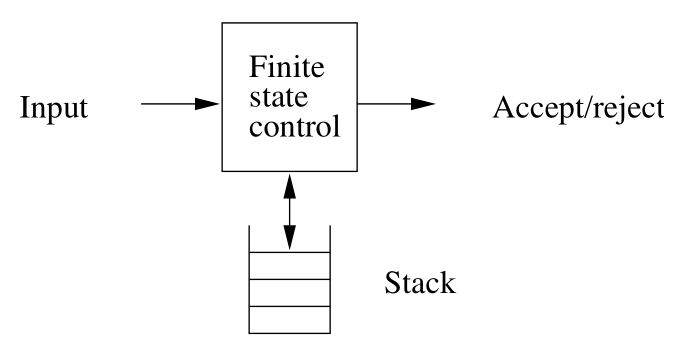
\includegraphics[scale=0.4]{files/pushDown.PNG}
                
    \end{columns}
    
    Expand the computation with a stack to a linear structure:
    \begin{itemize}
        \item[$X$] symbol pushed
        \item[$X^{-1}$] symbol popped
    \end{itemize}

    Pushing and popping form a pair that behaves like parentheses:
    $$
    \underbrace{ZZ^{-1}}\underbrace{B\underbrace{AA^{-1}}\underbrace{CC^{-1}}B^{-1}}
    $$

\end{frame}


\begin{frame}{The theorem}

    \begin{theorem}
        For any context-free language $L$ there exist a regular language $R$, a Dyck language $D$ and a homomorphism $h$ s.t. $L=h(D\cap R)$.
    \end{theorem}
    
    \textbf{Proof:} Start with a PDA recognizing $L$, accepting by empty stack.
    First, convert to instructions of the form:
    $$
    \delta(q,a,Z)\in (p,w), \alert{|w|\leq 2}
    $$ 
    (Instructions pushing more symbols can be split using new states).
            
    Let $R^|$ consist of all expressions of the form 
    $$
    q^{-1}aa^{-1}Z^{-1}BAp
    $$ 
    for instruction $\delta(q,a,Z)\ni (p,AB)$, and similarly for instructions $\delta(q,a,Z)\in (p,A)$ and $\delta(q,a,Z)\in (p,\epsilon)$. (For $a=\epsilon$ omit $aa^{-1}$.)
    
Now define the regular language as $R=Z_0q_0(R^|)^*Q^{-1}$.
    
    
    

\end{frame}


\begin{frame}
    \frametitle{Proof cont'd}

    The Dyck language $D$ is over the alphabet
    $$
    \Sigma\cup \Sigma^{-1} \cup Q\cup Q^{-1}\cup \Gamma\cup \Gamma^{-1}
    $$

    The language $D\cap R=D\cap Z_0q_0(R^|)^*Q^{-1}$ describes valid computations, e.g.
    $$
    \underbrace{Z_0\overbrace{q_0q_0^{-1}}aa^{-1}Z_0^{-1}}\underbrace{B\underbrace{A\overbrace{pp^{-1}}bb^{-1}A^{-1}}\overbrace{qq^{-1}}cc^{-1}B^{-1}}\overbrace{rr^{-1}}
    $$

    The homomorphism $h$ selects the input word being read:
      
    \begin{center}
        \begin{tabular}{l l}
            $h(a)=a$ & for input symbols $a\in\Sigma$\\
            $h(y)=\epsilon$ & for all other symbols
        \end{tabular}
    \end{center}    
    \hfill\qedsymbol

\end{frame}


\begin{frame}{Summary of Lecture 9}

    \begin{itemize}        
        \item Closure properties of context-free languages (including substitution, homomorphism, inverse homomorphism)
        \item Also closure properties of deterministic CFLs
        \item Dyck languages, a characterization of context-free languages
    \end{itemize}

\end{frame}



\end{document}